% Build the test insert first: platex -interaction=nonstopmode -halt-on-error smalltest1_review.tex
% Then: dvipdfmx smalltest1_review.dvi
% Build in this directory: pdflatex -interaction=nonstopmode -halt-on-error class2_handout.tex
\documentclass[a4paper,10pt,pdflatex,ja=standard,jafont=ipaex-type1,
  magstyle=real,scale=1]{bxjsarticle}
\usepackage{lmodern}
\usepackage{amsmath,amssymb,mathtools}
\usepackage{geometry}
\geometry{reset,left=22mm,right=22mm,top=20mm,bottom=17mm,
  headheight=13pt,headsep=6mm,footskip=10mm}
\usepackage{xcolor}
\usepackage{enumitem}
\usepackage{array,booktabs,tabularx}
\usepackage{fancyhdr}
\usepackage{lastpage}
\usepackage{pdfpages}

\definecolor{ink}{HTML}{193A5C}
\definecolor{accent}{HTML}{237D82}
\definecolor{soft}{HTML}{EAF3F3}
\definecolor{muted}{HTML}{52616B}
\newcommand{\coursename}{解析学 II}
\newcommand{\handoutnumber}{2}
\pagestyle{fancy}
\fancyhf{}
\fancyhead[L]{\small\color{ink}\coursename{}・授業要約と演習}
\fancyhead[R]{\small\color{ink}第\handoutnumber 回}
\fancyfoot[C]{\small\color{ink}\thepage/\pageref{LastPage}}
\renewcommand{\headrulewidth}{0.3pt}
\setlength{\parindent}{0pt}
\setlength{\parskip}{2pt}
\setlength{\abovedisplayskip}{5pt}
\setlength{\belowdisplayskip}{5pt}
\setlength{\abovedisplayshortskip}{3pt}
\setlength{\belowdisplayshortskip}{4pt}
\setlist[itemize]{leftmargin=1.8em,itemsep=1pt,topsep=2pt,parsep=0pt}

\newcommand{\handouttitle}[1]{%
  \begin{center}
    {\Large\color{ink}#1}\par\vspace{3mm}
    {\color{accent}\rule{0.88\linewidth}{0.7pt}}
  \end{center}\vspace{-2mm}}
\newcommand{\handout}[2]{%
  \renewcommand{\handoutnumber}{#1}%
  \handouttitle{第#1回\quad #2}}
\newcommand{\topic}[1]{\par\vspace{5pt}%
  {\large\sffamily\mdseries\color{accent}#1}\par\vspace{2pt}}
\newcommand{\keybox}[1]{\par\vspace{3pt}\begingroup
  \setlength{\fboxsep}{4pt}%
  \colorbox{soft}{\parbox{\dimexpr\linewidth-2\fboxsep\relax}{\small #1}}%
  \endgroup\par\vspace{2pt}}
\newenvironment{problems}
  {\begin{enumerate}[leftmargin=2em,itemsep=3pt,topsep=3pt,parsep=0pt,
    font=\color{accent}]}
  {\end{enumerate}}


\newcommand{\examplelabel}[1]{{\sffamily\mdseries\color{ink}#1}}
\newcommand{\problemspace}{\par\vspace{3mm}}
\newcommand{\exercises}{%
  {\color{accent}\hrule height 0.7pt}\vspace{3pt}%
  \topic{演習問題（6題）}%
}

% Keep each question together with its answer.
\newcommand{\feedback}[2]{%
  \par\addvspace{5pt}\noindent\begin{minipage}{\linewidth}%
  {\color{ink}Q. #1}\par\vspace{1pt}%
  {\color{accent}A. }#2%
  \end{minipage}\par}
% The insert uses the small-test class and shared style; apply common pagination here.
\fancypagestyle{smalltestpages}{%
  \fancyhf{}%
  \fancyhead[L]{\small\color{ink}\coursename{}・小テスト}%
  \fancyhead[R]{\small\color{ink}第1回}%
  \fancyfoot[C]{\small\color{ink}\thepage/\pageref{LastPage}}%
  \renewcommand{\headrulewidth}{0.3pt}}

\begin{document}
\fontsize{10pt}{13.5pt}\selectfont
\setlength{\abovedisplayskip}{4pt}
\setlength{\belowdisplayskip}{4pt}

\fancyhead[L]{\small\color{ink}\coursename{}・フィードバック}
\handout{2}{前回のコメントへのフィードバック}
\topic{逆関数・逆三角関数について}

\feedback{逆関数はどっちがどっちかわからなくなる}{%
$g$ が $f$ の逆関数なら、$f$ も $g$ の逆関数です。
$y=f(x)$ と $x=g(y)$ は同じ対応を、逆向きに見ているので区別する必要はないとおもいます。重要なのはどの関数の逆関数をみているかということですね。
}

\feedback{$\pm \sqrt{}$は逆関数ではないか}{%
その通りです！$\sqrt{}$がそもそも$x^2$の逆関数として定義されます。（授業ではふれませんでしたが）}

\feedback{問１で$\sqrt{y-1}\geq 0$より$y\geq 1$が定義域と解答でかいたが、必要か？}{%
ぜひ書いてください！できれば$f,g$の定義域を明確に書くほうが良いです。（書かなくてもこの授業では正しいとする予定ではありますが）}

\feedback{三角関数の逆関数は定義域を毎回かくべきか？}{%
問題によると思います。定義域をかけと明言されていなければ書かなくてもよいと思います。}

\feedback{逆関数を求める問題で、$x=y$の式のあと$x$と$y$を入れ替える必要があるか?}{%
どちらでも大丈夫です。}

\feedback{逆三角関数の定義域はなぜ$[-\pi/2,\pi/2]$にするのか？}{%
これは大きな理由はなく$[-3\pi/2,-\pi/2]$としてもよいのですが、それぞれの人が違う定義をつかっているとわかりにくいので統一しているという認識です。}

\feedback{逆三角関数はなぜ大文字でかく？}{%
これは指定教科書独特な記号ですね。普通は$\arcsin$のように書きます。}

\feedback{問１が自信ない}{%
あっています！}

\feedback{高校生の時に参考書に逆三角関数の積分が書いてあったが理解不能。今回はリベンジ}{%
ぜひリベンジしてください}

\topic{学習の進め方について}
\feedback{授業の時は理解できてるが、次の週で忘れる}{%
授業前に１０分程度でいいので復習するといいと思います。（小テスト中だと時間に限りがあるので）}

\feedback{ここからどんな難しい問題がでるかと思うと眠れない}{%
大丈夫ですのでよく寝てください}

\newpage
\handouttitle{第2回\quad フィードバック（つづき）}
\topic{数学・AI・これからのこと}

\feedback{ほかの未解決問題も知りたい。}{%
今回紹介したのは七武海みたいなもので、実はその上の始皇帝みたいのが存在します。コラッツ予想やゴールドバッハ予想などは大学の数学の知識がなくても理解できるので、どこかで話したいですね。}

\feedback{数学の問題はAIがすべて解いてしまうのか？}{%
AIに関する予想はだいたい外れるのでかなりリスクがありますが、ミレニアム問題でいうとリーマン予想、ホッジ予想、BSD予想は年内に解かれる可能性はそれなりにあると思います。個人的には$P\neq NP$問題とヤンミルズは当分解かれないかなと思っています。理由は、$P\neq NP$は証明不可能問題である可能性があるのと、ヤンミルズは問題の定式化が明確にされていないからです。ちなみに20世紀中盤にチューリングの面白い研究があって、かなり大雑把に言うと機械にも"解けない"問題があるというものです。ただし人間が興味のある問題が"解けない"問題に入っているかが良くわかっていないですが、、}

\feedback{今回のミレニアム問題の解決で、人間に求められるものがかなり変わった気がした。}{%
ここから２，３年で問題解決（数学に限らず広い意味で）はAIのほうが得意になる可能性は十分あるとは思います。個人的には、問題解決でない単純に興味があるとか面白いからという理由の社会活動が許される社会であってほしいなとは思いますが、こういう社会システムである以上難しいのかもしれません、、}

\feedback{今後ＡＩに制約をかけていくか、世界のためにそのままにしておくか}{%
最近議論されるようになっていますが、私は世界の発展のために積極的に制約をかけていくべきだと思います。ここでいう制約というのは、ＡＩの性能向上をやめるということではなく、できたＡＩに対してなにが実行できるかということを明確に制限するという意味です。まったく制約のないAIは、現在サイバーテロが頻発しているように必ず大きな問題を引き起こすと思います。}

\feedback{Qwen 3.5の精度がよくなってうれしい}{%
Qwen使っているのは珍しいですね笑}

\feedback{先週はOpenAIが多くの数学の問題を発表した}{%
実は自分が今年取り組もうと思っていた問題が入ってて、悲しくなりました。まだ証明が正しいか確認されているわけではないので今読んでいるのですが、証明は宇宙人が書いたような文章で理解には至っていないです。}

\feedback{ＡＩが発展しても人間が研究しなきゃいけない領域があると知れて安心した。}{%
そうですね。ＡＩ安全性、実験安全性、ソフトウェア安全性は今後も必ず人間がやるようにしないといけないですね。}

\feedback{ＡＩが発達した未来に自分はなにをすべきか}{%
何かを成したい場合は、新しいことに挑戦するしかないのかなと思ったりします。}

\topic{授業の予定・そのほか}
\feedback{中間テストの日程がきになる。}{%
今のところ第八回の予定です。（何日になるかがわかっていないですが）}

\feedback{四限になりませんか}{%
偉い人に相談してみます。（今年はもう遅いですけど）}

\feedback{昨日のドラマで関講和がでてきた。}{%
「いろはの恋は時代（とき）をかける」という作品ですか。面白そうですね、拝聴したいと思います}

\feedback{朝ごはんはごはんかパンか?　何時におきたか?}{%
ヨーグルトとバナナですね。７時です。}


\clearpage
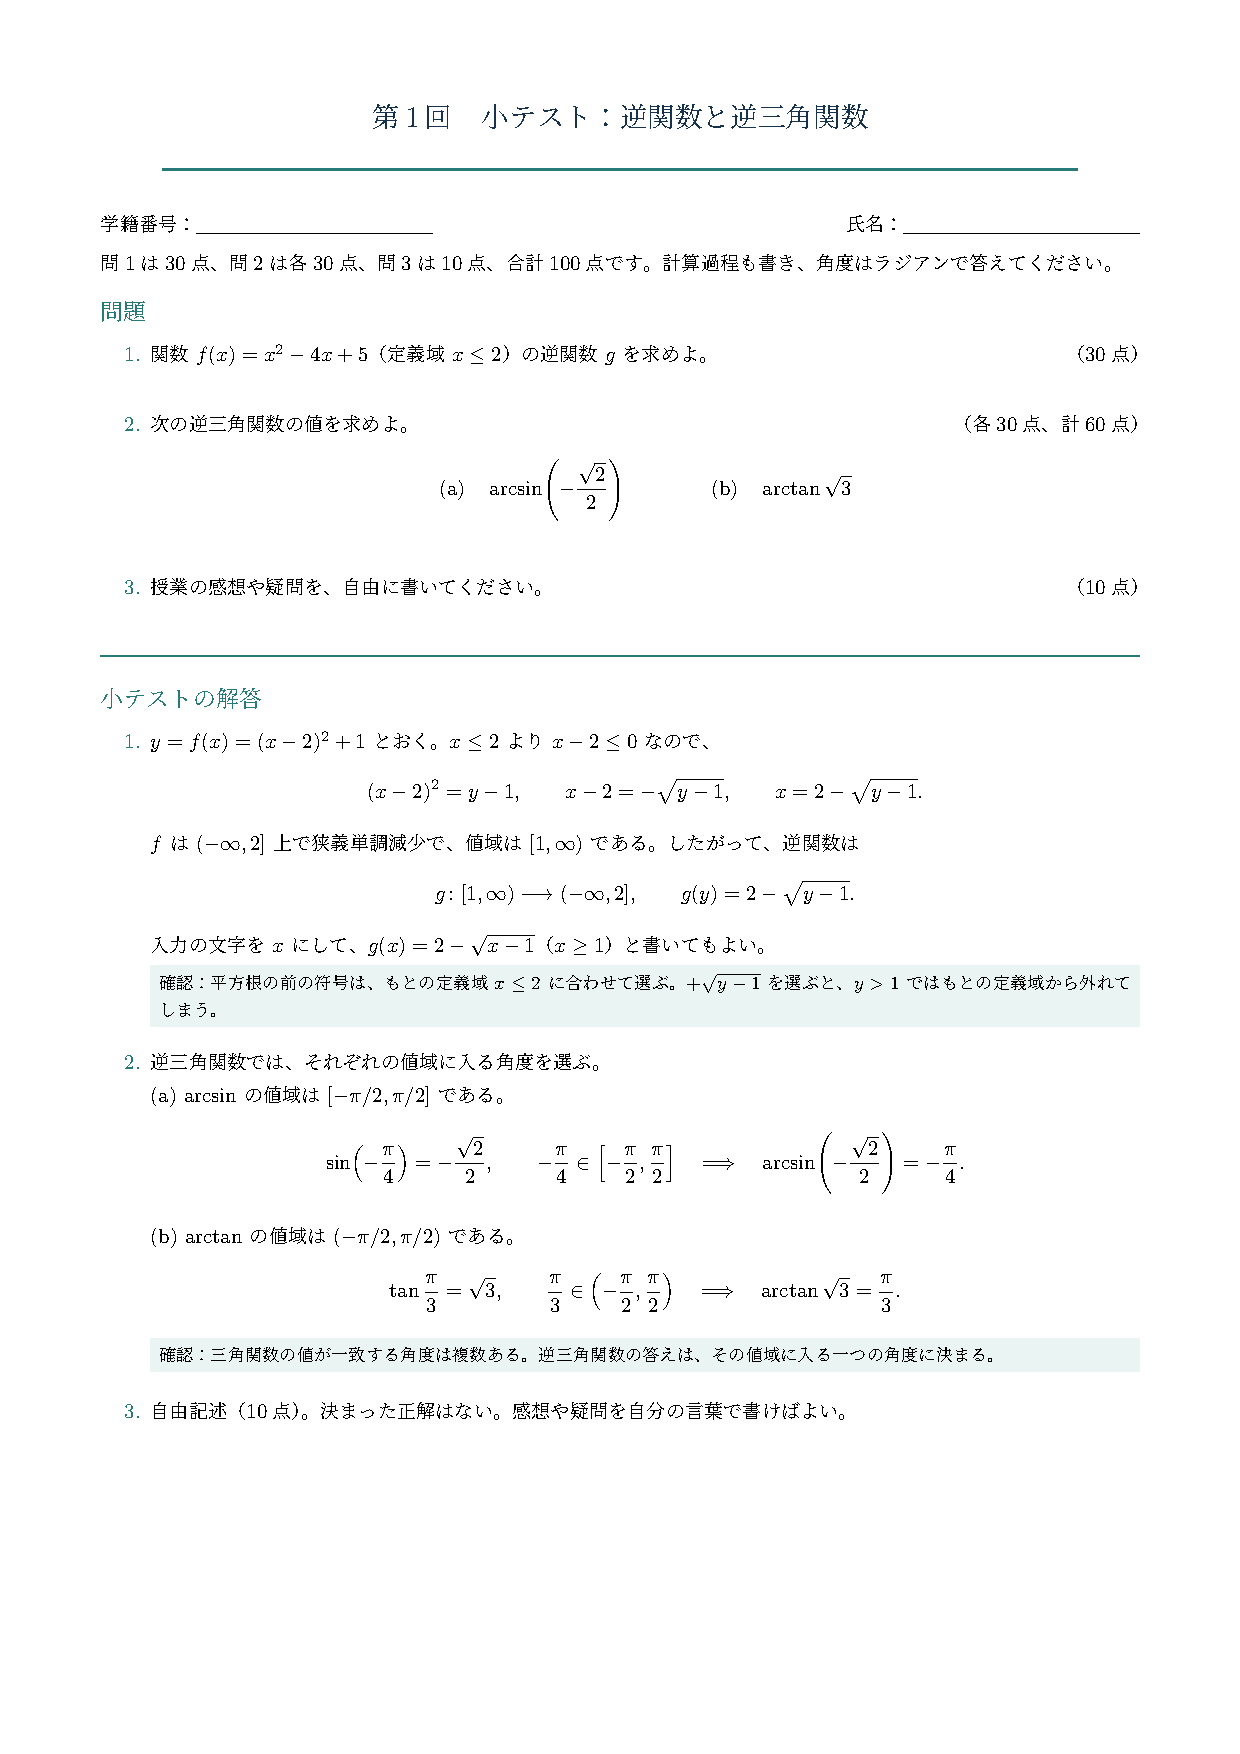
\includepdf[pages=-,pagecommand={\thispagestyle{smalltestpages}}]{smalltest1_review.pdf}
\fancyhead[L]{\small\color{ink}\coursename{}・授業要約と演習}
% The lesson summary, exercises and answers occupy the final three pages.
\handout{2}{有理関数の積分}

$P,Q$ は実係数多項式（$Q\not\equiv0$）とし、$Q(x)\ne0$ の各区間で積分する。
$C$ は区間ごとに選ぶ積分定数、$\log$ は自然対数 を表す。

\topic{割り算で「多項式＋真分数」にする}
$\deg$ は多項式の次数（$\deg0=-\infty$）を表す。
$\deg P\ge\deg Q$ なら、商 $H$ と余り $R$ を求めて
$$
 P=HQ+R,\qquad \frac{P}{Q}=H+\frac{R}{Q}
 \qquad(R=0\ \text{または}\ \deg R<\deg Q).
$$


\topic{分母を因数分解する}
分母を実一次式と既約二次式の積にする。
$q(x)=x^2+ax+b$ は $D=a^2-4b$ で分類する。
$$
 \begin{array}{c|l|l}
 D & \text{分母の扱い方} & \text{例}\\ \hline
 D>0 & \text{異なる一次式の積にする} & x^2-3x+2=(x-1)(x-2)\\[2pt]
 D=0 & \text{一次式の2乗になる} & x^2+2x+1=(x+1)^2\\[2pt]
 D<0 & \text{平方完成して二次式のまま残す} & x^2+4x+13=(x+2)^2+9
 \end{array}
$$
$D<0$ では $q(x)=(x+a/2)^2+c^2$、$c=\sqrt{b-a^2/4}>0$ となり、一次式に分解できない（既約）。

\topic{部分分数の形を決め、係数を求める}
真分数では、一次因子には定数、既約二次因子には一次以下の式を分子に置く。
因子が $m$ 乗（$m\ge1$ の整数）なら、1乗から $m$ 乗までの項をすべて用意する。
$$
 \begin{array}{c|l}
 \text{分母の因子} & \text{用意する項（係数は未定の実数）}\\ \hline
 (x-\alpha)^m & \dfrac{A_1}{x-\alpha}+\dfrac{A_2}{(x-\alpha)^2}
   +\cdots+\dfrac{A_m}{(x-\alpha)^m}\\[7pt]
 (x^2+ax+b)^m\ (D<0) & \dfrac{B_1x+E_1}{q(x)}
   +\dfrac{B_2x+E_2}{(x^2+ax+b)^2}+\cdots+\dfrac{B_mx+E_m}{(x^2+ax+b)^m}
 \end{array}
$$
両辺に分母を掛けて多項式の恒等式にし、実零点の代入と係数比較で係数を求める。

\examplelabel{例：重なった一次因子}
$\dfrac1{x(x-1)^2}=\dfrac Ax+\dfrac B{x-1}+\dfrac E{(x-1)^2}$ とおくと
$$
 1=A(x-1)^2+Bx(x-1)+Ex.
$$
$x=0,1$ の代入から $A=E=1$、$x^2$ の係数比較から $A+B=0$、よって $B=-1$。

\topic{各項を基本公式で積分する}
以下、$\alpha,p\in\mathbb R$、$c>0$、整数 $n\ge2$ とし、表では $+C$ を省略する。
$$
 \begin{array}{l|l}
 \text{一次因子の公式} & \text{二次式の公式}\\ \hline
 \displaystyle\int\frac{dx}{x-\alpha}=\log|x-\alpha|
   & \displaystyle\int\frac{dx}{(x+p)^2+c^2}=\frac1c{\rm Tan}^{-1} \frac{x+p}{c}\\[8pt]
 \displaystyle\int\frac{dx}{(x-\alpha)^n}=-\frac1{(n-1)(x-\alpha)^{n-1}}
   & \displaystyle\int\frac{q'(x)}{q(x)}\,dx=\log|q(x)|
 \end{array}
$$
分子が一次式なら「分母の微分の定数倍＋定数」に分ける。
たとえば $x+5=\tfrac12(2x+4)+3$ より、$\mathbb R$ 上で
$$
 \int\frac{x+5}{x^2+4x+13}\,dx
 =\frac12\log(x^2+4x+13)+{\rm Tan}^{-1} \frac{x+2}{3}+C.
$$
上の部分分数の例は、$(-\infty,0)$、$(0,1)$、$(1,\infty)$ の各区間で
$$
 \int\frac{dx}{x(x-1)^2}=\log|x|-\log|x-1|-\frac1{x-1}+C.
$$
既約二次因子の累乗は、平方完成の後に部分積分で指数を下げて扱う（演習6）。

\newpage
% Keep the worked examples in the upper half of page 2.
\noindent\begin{minipage}[b][\dimexpr0.5\textheight-\parskip\relax][t]{\linewidth}
\topic{例題：解き方の流れ}
\examplelabel{例題1　割り算が必要な場合}\par
分子・分母がともに2次なので、まず割り算する。
$$
 \frac{x^2+1}{x(x-1)}=1+\frac{x+1}{x(x-1)},\qquad
 \frac{x+1}{x(x-1)}=\frac Ax+\frac B{x-1}.
$$
分母を払うと $x+1=A(x-1)+Bx$。
$x=0$ で $A=-1$、$x=1$ で $B=2$ だから
$$
 \int\frac{x^2+1}{x(x-1)}\,dx=x-\log|x|+2\log|x-1|+C.
$$

\medskip
\examplelabel{例題2　一次因子と既約二次因子がある場合}
$$
 \frac{x^2+x+1}{(x-1)(x^2+1)}=\frac A{x-1}+\frac{Bx+E}{x^2+1}.
$$
分母を払うと $x^2+x+1=A(x^2+1)+(Bx+E)(x-1)$。
$x=1$ の代入、$x^2$ と定数項の比較から
$$
 3=2A,\qquad 1=A+B,\qquad 1=A-E
 \quad\Longrightarrow\quad A=\frac32,\ B=-\frac12,\ E=\frac12.
$$
二次式の分子を分けて積分すると
$$
 \begin{aligned}
 \int\frac{x^2+x+1}{(x-1)(x^2+1)}\,dx
 &=\int\left(\frac{3}{2(x-1)}-\frac14\frac{2x}{x^2+1}
      +\frac1{2(x^2+1)}\right)dx\\
 &=\frac32\log|x-1|-\frac14\log(x^2+1)+\frac12{\rm Tan}^{-1}  x+C.
 \end{aligned}
$$
\end{minipage}\par\nointerlineskip
% Keep exercises and writing space in the lower half of page 2.
\noindent\begin{minipage}[b][0.5\textheight][t]{\linewidth}
\exercises
\begin{problems}
\item $\displaystyle\int\frac{dx}{x-2}$ を求めよ。
\problemspace

\item $\displaystyle\int\frac{dx}{(x+1)^3}$ を求めよ。
\problemspace

\item 平方完成して積分せよ。((b) は分子を「分母の微分の定数倍＋定数」に分けよ。)
$$
 \text{(a)}\quad\int\frac{dx}{x^2+2x+5},\qquad
 \text{(b)}\quad\int\frac{x+2}{x^2+x+3}\,dx.
$$
\problemspace

\item 部分分数分解して積分せよ:
$$
 \text{(a)}\quad\int\frac{dx}{x(x+1)^2},\qquad
 \text{(b)}\quad\int\frac{x+1}{x(x^2+1)}\,dx.
$$
\problemspace

\item $\displaystyle\int\frac{x^3}{x^2+1}\,dx$ を求めよ。（ヒント：まず割り算。）
\problemspace

\item 整数 $n\ge1$、$x\in\mathbb R$ に対し、$I_n(x)=\displaystyle\int_0^x\frac{dt}{(1+t^2)^n}$ とおく。
部分積分で $I_{n+1}$ と $I_n$ の漸化式を導き、すべての $I_n$ が順に求まることを示せ。
\problemspace
\end{problems}
\end{minipage}
\newpage
\handouttitle{第2回\quad 演習問題の解答}
{\small 以下、$C$ は積分定数であり、分母の零点で区切られる区間ごとに異なってよい。}\par
\begin{problems}
\setlength{\itemsep}{5pt}
\item $x<2$ または $x>2$ の各区間で
$$
 \int\frac{dx}{x-2}=\log|x-2|+C.
$$
$x<2$ では $\log|x-2|=\log(2-x)$ だから、微分すると
$-1/(2-x)=1/(x-2)$ となり、この区間でも正しい。

\item $x<-1$ または $x>-1$ の各区間で、$n=3$ の公式より
$$
 \int\frac{dx}{(x+1)^3}=-\frac1{2(x+1)^2}+C.
$$
べき乗の公式 $-1/\{(n-1)(x-\alpha)^{n-1}\}$ に $n=1$ を代入すると
分母が0になる。$n=1$ の場合は別に計算し、$\log|x-\alpha|+C$ を用いる。

\item どちらの分母もすべての実数 $x$ で正なので、区間は $\mathbb R$ でよい。
(a) $x^2+2x+5=(x+1)^2+4$ より
$$
 \int\frac{dx}{x^2+2x+5}=\frac12{\rm Tan}^{-1} \frac{x+1}{2}+C.
$$
(b) $q(x)=x^2+x+3=(x+\tfrac12)^2+\tfrac{11}{4}$ とおく。
$x+2=\tfrac12q'(x)+\tfrac32$ と分けると
$$
 \int\frac{x+2}{x^2+x+3}\,dx
 =\frac12\log(x^2+x+3)+\frac3{\sqrt{11}}{\rm Tan}^{-1} \frac{2x+1}{\sqrt{11}}+C.
$$

\item (a) 分母を払った恒等式は
$$
 1=A(x+1)^2+Bx(x+1)+Ex.
$$
$x=0,-1$ の代入と係数比較から $A=1$、$B=E=-1$ を得る。したがって
$$
 \begin{aligned}
 \frac1{x(x+1)^2}&=\frac1x-\frac1{x+1}-\frac1{(x+1)^2},\\
 \int\frac{dx}{x(x+1)^2}&=\log|x|-\log|x+1|+\frac1{x+1}+C.
 \end{aligned}
$$
区間は $(-\infty,-1)$、$(-1,0)$、$(0,\infty)$ のいずれかである。
(b) 恒等式と係数は
$$
 x+1=A(x^2+1)+(Bx+E)x,\qquad A=1,\quad B=-1,\quad E=1.
$$
よって $x<0$ または $x>0$ の各区間で
$$
 \begin{aligned}
 \frac{x+1}{x(x^2+1)}&=\frac1x+\frac{-x+1}{x^2+1},\\
 \int\frac{x+1}{x(x^2+1)}\,dx
 &=\log|x|-\frac12\log(x^2+1)+{\rm Tan}^{-1}  x+C.
 \end{aligned}
$$

\item 除法により $x^3=x(x^2+1)-x$ だから、$\mathbb R$ 上で
$$
 \int\frac{x^3}{x^2+1}\,dx
 =\int\left(x-\frac{x}{x^2+1}\right)dx
 =\frac{x^2}{2}-\frac12\log(x^2+1)+C.
$$

\item $x\in\mathbb R$ で、$I_n$ を部分積分すると
$$
 \begin{aligned}
 I_n(x)&=\left[\frac{t}{(1+t^2)^n}\right]_0^x
       +2n\int_0^x\frac{t^2}{(1+t^2)^{n+1}}\,dt\\
 &=\frac{x}{(1+x^2)^n}+2n\bigl(I_n(x)-I_{n+1}(x)\bigr).
 \end{aligned}
$$
$t^2=(1+t^2)-1$ を用いた。整理して、積分定数を含まない漸化式を得る。
$$
 I_{n+1}(x)=\frac{x}{2n(1+x^2)^n}+\frac{2n-1}{2n}I_n(x).
$$
$I_1(x)={\rm Tan}^{-1}  x$ から出発し、この式で $I_2,I_3,\ldots$ が順に求まる。
帰納法により、各 $I_n$ は有理関数と ${\rm Tan}^{-1}  x$ の定数倍の和になる。
不定積分の答えは $I_n(x)+C$ である。
\end{problems}
\end{document}
